\documentclass[letterpaper, 12pt]{article}


\usepackage{amsmath}
\usepackage{ragged2e}
\usepackage{graphicx}
\usepackage{pdfpages}

\topmargin 0.0cm
\oddsidemargin 0.2cm
\textwidth 16cm 
\textheight 21cm
\footskip 1.0cm


%The next command sets up an environment for the abstract to your paper.

\newenvironment{sciabstract}{%
\begin{quote} \bf}
{\end{quote}}


% If your reference list includes text notes as well as references,
% include the following line; otherwise, comment it out.

\renewcommand\refname{References and Notes}

% The following lines set up an environment for the last note in the
% reference list, which commonly includes acknowledgments of funding,
% help, etc.  It's intended for users of BibTeX or the {thebibliography}
% environment.  Users who are hand-coding their references at the end
% using a list environment such as {enumerate} can simply add another
% item at the end, and it will be numbered automatically.

\newcounter{lastnote}
\newenvironment{scilastnote}{%
\setcounter{lastnote}{\value{enumiv}}%
\addtocounter{lastnote}{+1}%
\begin{list}%
{\arabic{lastnote}.}
{\setlength{\leftmargin}{.22in}}
{\setlength{\labelsep}{.5em}}}
{\end{list}}


% Include your paper's title here
\begin{document}
\large\title{{Sistema de Lorenz}} 
\author{L.M. Duque Valencia,$^{1}$ L. Del Castillo Detoeuf,$^{2}$ J.F. Reyes Botero$^{3}$}
\date{}
\maketitle
\centering\normalsize{$^{1, 2, 3}$Universidad Nacional de Colombia}\\
\centering\normalsize{Departamento de F\'isica, Facultad de Ciencias}\\
\centering\normalsize{Programaci\'on e Introducci\'on a los M\'etodos Num\'ericos}\\
\centering\normalsize{\{$^{1}$lmduquev, $^{2}$ldeld, $^{3}$jfreyesb\}@unal.edu.co\\

\baselineskip18pt



\begin{sciabstract}
  Este proyecto se propone estudiar gráficamente el sistema de ecuaciones diferenciales conocido como sistema de Lorenz haciendo uso del método de aproximación de Runge-Kutta 4 y de herramientas computacionales estudiadas durante el semestre. En primer lugar se modeló el sistema usando un programa en lenguaje en C++, se graficaron las soluciones obtenidas en 3D y las proyecciones sobre los tres planos principales usando el programa Gnuplot. Finalmente, se modificaron ligeramente las condiciones iniciales del modelo para comprobar que se trata de un sistema caótico.
\end{sciabstract}



% In setting up this template for *Science* papers, we've used both
% the \section* command and the \paragraph* command for topical
% divisions.  Which you use will of course depend on the type of paper
% you're writing.  Review Articles tend to have displayed headings, for
% which \section* is more appropriate; Research Articles, when they have
% formal topical divisions at all, tend to signal them with bold text
% that runs into the paragraph, for which \paragraph* is the right
% choice.  Either way, use the asterisk (*) modifier, as shown, to
% suppress numbering.

\section*{Introducci\'on}

\justify
El sistema de Lorenz, introducido por Edward Lorenz en 1963, es un modelo tridimensional de la dinámica atmosférica terrestre expresado en sistema no lineal y determinista de tres ecuaciones diferenciales. El modelo se basa en tres parámetros y las condiciones iniciales del sistema de ecuaciones: $\sigma$ (número de Prant), $\rho$ (número de Rayleigh) y $\beta$.
El sistema se expresa de la siguiente forma:
\begin{align}
\dot{X} = \sigma (Y-X)\\
\dot{Y} = X(\rho - Z)\\
\dot{Z} = XY - \beta Z
\end{align}
Donde $X$ es la velocidad de la corriente de convección, $Y$ es proporcional a la diferencia de temperatura entre  corrientes de convección ascendetes y descendentes y $Z$ es la desviación de la temperaratura respecto a la dependencia lineal de la altura. Este sistema es de gran interés matemático pues para ciertos valores de los parámetros muestra un comportamiento caótico con un atractor conocido como "\textit{Mariposa de Lorenz}". 


\section*{Programaci\'on}

\justify
El programa implementado para aproximar las soluciones del sistema de Lorenz consiste en 5 funciones y una estructura, e imprime los valores sucesivos de $X$, $Y$, y $Z$ cada $10^{-4}$ segundos en un rango de tiempo de 0 a 50. En primer lugar, se declara una estructura con tres variables \textit{double} $x_0$, $y_0$, y $z_0$ que representan los valores de las ecuaciones en un tiempo $t$:\\
\begin{center}
\includegraphics{estructura.png}\\
\end{center}
 En seguida, implementamos tres funciones \textit{ff, gg} y \textit{hh}, una para cada ecuación diferencial del sistema de Lorenz. Usamos los siguientes valores para los parámetros del sistema: $\sigma = 10$, $\rho = \frac{8}{3}$, $\beta = 28$. 
\begin{center}
 \includegraphics{funciones.png}
\end{center}

Después introducimos una función que realice los cálculos del método RK4. Esta función toma como argumentos las variables $x_0$, $y_0$, y $z_0$ en un tiempo $t_i$ y usa un $\Delta t = 10^{-4}$ y las tres funciones de las ecuaciones para aproximar los valores del sistema en el tiempo $t_{i+1} = t_i + \Delta t$. La función finaliza modificando los valores $x_0$, $y_0$, y $z_0$ de la estructura por los calculados con el método RK4.

Finalmente, usamos la función \textit{main} para asignar los valores de las condiciones iniciales a las variables de la estructura. Luego iteramos la función RK4 desde $t = 0$ a $t = 50$, imprimiendo a cada paso los resultados de $x_0$, $y_0$, y $z_0$. Estos datos son guardados en un archivo de texto para ser graficados usando \textbf{Gnuplot}.

Para obtener los datos para graficar las proyecciones sobre los tres planos $XY$, $XZ$ y $YZ$, y la gráfica de $Y$ en funci\'on de $t$, usamos el mismo programa modificando \'unicamente la \'ultima l\'inea del ciclo \textit{for} para que imprima s\'olo los valores necesarios ($X$ y $Y$, $X$ y $Z$, $Y$ y $Z$, y $t$ y $Y$, respectivamente):


\section*{Graficar los resultados}

\justify
Al graficar los resultados en \textbf{Gnuplot}, s\'olo se usaron uno de cada 10 datos para que la talla de los archivos no fuera demasiado grande. Usamos el siguiente c\'odigo para generar los pdf:

Obtuvimos la siguiente "Mariposa de Lorenz":
%\begin{center}
%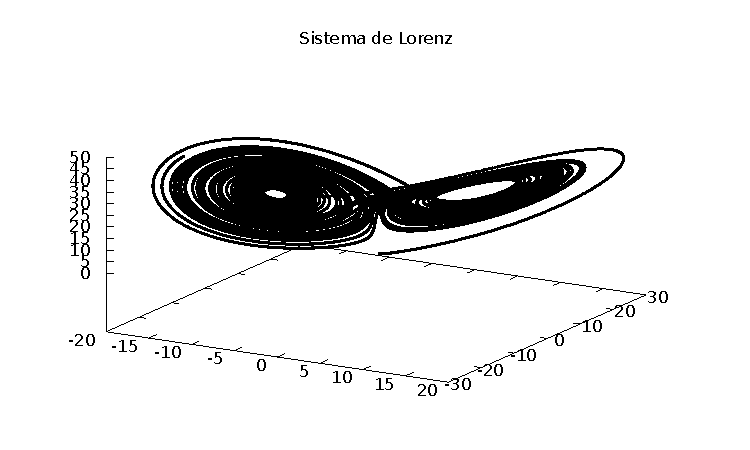
\includepdf[width=\textwidth]{lorenz.pdf}
%\end{center}

Para visualizar mejor la forma tridimensional de la "\textit{mariposa}", usamos la terminal de \textit{gif} de Gnuplot para animar la rotaci\'on sobre el eje $z$ de la gr\'afica (ver "mariposa.gif" en el repositorio). Usamos los siguientes comandos de Gnuplot para siular la rotaci\'on:



\section*{Formatting Citations}

Citations can be handled in one of three ways.  The most
straightforward (albeit labor-intensive) would be to hardwire your
citations into your \LaTeX\ source, as you would if you were using an
ordinary word processor.  Thus, your code might look something like
this:


\begin{quote}
\begin{verbatim}
However, this record of the solar nebula may have been
partly erased by the complex history of the meteorite
parent bodies, which includes collision-induced shock,
thermal metamorphism, and aqueous alteration
({\it 1, 2, 5--7\/}).
\end{verbatim}
\end{quote}


\noindent Compiled, the last two lines of the code above, of course, would give notecalls in {\it Science\/} style:

\begin{quote}
\ldots thermal metamorphism, and aqueous alteration ({\it 1, 2, 5--7\/}).
\end{quote}

Under the same logic, the author could set up his or her reference list as a simple enumeration,

\begin{quote}
\begin{verbatim}
{\bf References and Notes}

\begin{enumerate}
\item G. Gamow, {\it The Constitution of Atomic Nuclei
and Radioactivity\/} (Oxford Univ. Press, New York, 1931).
\item W. Heisenberg and W. Pauli, {\it Zeitschr.\ f.\ 
Physik\/} {\bf 56}, 1 (1929).
\end{enumerate}
\end{verbatim}
\end{quote}

\noindent yielding

\begin{quote}
{\bf References and Notes}

\begin{enumerate}
\item G. Gamow, {\it The Constitution of Atomic Nuclei and
Radioactivity\/} (Oxford Univ. Press, New York, 1931).
\item W. Heisenberg and W. Pauli, {\it Zeitschr.\ f.\ Physik} {\bf 56},
1 (1929).
\end{enumerate}
\end{quote}

That's not a solution that's likely to appeal to everyone, however ---
especially not to users of B{\small{IB}}\TeX\ \cite{inclme}.  If you
are a B{\small{IB}}\TeX\ user, we suggest that you use the
\texttt{Science.bst} bibliography style file and the
\texttt{scicite.sty} package, both of which we are downloadable from our author help site
(http://www.sciencemag.org/about/authors/prep/TeX\_help/).  You can also
generate your reference lists by using the list environment
\texttt{\{thebibliography\}} at the end of your source document; here
again, you may find the \texttt{scicite.sty} file useful.

Whether you use B{\small{IB}}\TeX\ or \texttt{\{thebibliography\}}, be
very careful about how you set up your in-text reference calls and
notecalls.  In particular, observe the following requirements:

\begin{enumerate}
\item Please follow the style for references outlined at our author
  help site and embodied in recent issues of {\it Science}.  Each
  citation number should refer to a single reference; please do not
  concatenate several references under a single number.
\item Please cite your references and notes in text {\it only\/} using
  the standard \LaTeX\ \verb+\cite+ command, not another command
  driven by outside macros.
\item Please separate multiple citations within a single \verb+\cite+
  command using commas only; there should be {\it no space\/}
  between reference keynames.  That is, if you are citing two
  papers whose bibliography keys are \texttt{keyname1} and
  \texttt{keyname2}, the in-text cite should read
  \verb+\cite{keyname1,keyname2}+, {\it not\/}
  \verb+\cite{keyname1, keyname2}+.
\end{enumerate}

\noindent Failure to follow these guidelines could lead
to the omission of the references in an accepted paper when the source
file is translated to Word via HTML.

\section*{Handling Math, Tables, and Figures}

Following are a few things to keep in mind in coding equations,
tables, and figures for submission to {\it Science}.

\paragraph*{In-line math.}  The utility that we use for converting
from \LaTeX\ to HTML handles in-line math relatively well.  It is best
to avoid using built-up fractions in in-line equations, and going for
the more boring ``slash'' presentation whenever possible --- that is,
for \verb+$a/b$+ (which comes out as $a/b$) rather than
\verb+$\frac{a}{b}$+ (which compiles as $\frac{a}{b}$).  Likewise,
HTML isn't tooled to handle certain overaccented special characters
in-line; for $\hat{\alpha}$ (coded \verb+$\hat{\alpha}$+), for
example, the HTML translation code will return [\^{}$(\alpha)$].
Don't drive yourself crazy --- but if it's possible to avoid such
constructs, please do so.  Please do not code arrays or matrices as
in-line math; display them instead.  And please keep your coding as
\TeX-y as possible --- avoid using specialized math macro packages
like \texttt{amstex.sty}.

\paragraph*{Displayed math.} Our HTML converter sets up \TeX\
displayed equations using nested HTML tables.  That works well for an
HTML presentation, but Word chokes when it comes across a nested
table in an HTML file.  We surmount that problem by simply cutting the
displayed equations out of the HTML before it's imported into Word,
and then replacing them in the Word document using either images or
equations generated by a Word equation editor.  Strictly speaking,
this procedure doesn't bear on how you should prepare your manuscript
--- although, for reasons best consigned to a note \cite{nattex}, we'd
prefer that you use native \TeX\ commands within displayed-math
environments, rather than \LaTeX\ sub-environments.

\paragraph*{Tables.}  The HTML converter that we use seems to handle
reasonably well simple tables generated using the \LaTeX\
\texttt{\{tabular\}} environment.  For very complicated tables, you
may want to consider generating them in a word processing program and
including them as a separate file.

\paragraph*{Figures.}  Figure callouts within the text should not be
in the form of \LaTeX\ references, but should simply be typed in ---
that is, \verb+(Fig. 1)+ rather than \verb+\ref{fig1}+.  For the
figures themselves, treatment can differ depending on whether the
manuscript is an initial submission or a final revision for acceptance
and publication.  For an initial submission and review copy, you can
use the \LaTeX\ \verb+{figure}+ environment and the
\verb+\includegraphics+ command to include your PostScript figures at
the end of the compiled PostScript file.  For the final revision,
however, the \verb+{figure}+ environment should {\it not\/} be used;
instead, the figure captions themselves should be typed in as regular
text at the end of the source file (an example is included here), and
the figures should be uploaded separately according to the Art
Department's instructions.


\section*{What to Send In}

What you should send to {\it Science\/} will depend on the stage your manuscript is in:

\begin{itemize}
\item {\bf Important:} If you're sending in the initial submission of
  your manuscript (that is, the copy for evaluation and peer review),
  please send in {\it only\/} a PostScript or PDF version of the
  compiled file (including figures).  Please do not send in the \TeX\ 
  source, \texttt{.sty}, \texttt{.bbl}, or other associated files with
  your initial submission.  (For more information, please see the
  instructions at our Web submission site,
  http://www.submit2science.org/ .)
\item When the time comes for you to send in your revised final
  manuscript (i.e., after peer review), we require that you include
  all source files and generated files in your upload.  Thus, if the
  name of your main source document is \texttt{ltxfile.tex}, you
  need to include:
\begin{itemize}
\item \texttt{ltxfile.tex}.
\item \texttt{ltxfile.aux}, the auxilliary file generated by the
  compilation.
\item A PostScript file (compiled using \texttt{dvips} or some other
  driver) of the \texttt{.dvi} file generated from
  \texttt{ltxfile.tex}, or a PDF file distilled from that
  PostScript.  You do not need to include the actual \texttt{.dvi}
  file in your upload.
\item From B{\small{IB}}\TeX\ users, your bibliography (\texttt{.bib})
  file, {\it and\/} the generated file \texttt{ltxfile.bbl} created
  when you run B{\small{IB}}\TeX.
\item Any additional \texttt{.sty} and \texttt{.bst} files called by
  the source code (though, for reasons noted earlier, we {\it
    strongly\/} discourage the use of such files beyond those
  mentioned in this document).
\end{itemize}
\end{itemize}

% Your references go at the end of the main text, and before the
% figures.  For this document we've used BibTeX, the .bib file
% scibib.bib, and the .bst file Science.bst.  The package scicite.sty
% was included to format the reference numbers according to *Science*
% style.


\bibliography{scibib}

\bibliographystyle{Science}



% Following is a new environment, {scilastnote}, that's defined in the
% preamble and that allows authors to add a reference at the end of the
% list that's not signaled in the text; such references are used in
% *Science* for acknowledgments of funding, help, etc.

\begin{scilastnote}
\item We've included in the template file \texttt{scifile.tex} a new
environment, \texttt{\{scilastnote\}}, that generates a numbered final
citation without a corresponding signal in the text.  This environment
can be used to generate a final numbered reference containing
acknowledgments, sources of funding, and the like, per {\it Science\/}
style.
\end{scilastnote}




% For your review copy (i.e., the file you initially send in for
% evaluation), you can use the {figure} environment and the
% \includegraphics command to stream your figures into the text, placing
% all figures at the end.  For the final, revised manuscript for
% acceptance and production, however, PostScript or other graphics
% should not be streamed into your compliled file.  Instead, set
% captions as simple paragraphs (with a \noindent tag), setting them
% off from the rest of the text with a \clearpage as shown  below, and
% submit figures as separate files according to the Art Department's
% instructions.


\clearpage

\noindent {\bf Fig. 1.} Please do not use figure environments to set
up your figures in the final (post-peer-review) draft, do not include graphics in your
source code, and do not cite figures in the text using \LaTeX\
\verb+\ref+ commands.  Instead, simply refer to the figure numbers in
the text per {\it Science\/} style, and include the list of captions at
the end of the document, coded as ordinary paragraphs as shown in the
\texttt{scifile.tex} template file.  Your actual figure files should
be submitted separately.



\end{document}




















